%==============================================================================
% tento soubor pouzijte jako zaklad
% this file should be used as a base for the thesis
% (c) 2008 Michal Bidlo
% E-mail: bidlom AT fit vutbr cz
% Šablonu upravil / template edited by: Ing. Jaroslav Dytrych, dytrych@fit.vutbr.cz
%==============================================================================
% kodovaní: UTF-8 (zmena prikazem iconv, recode nebo cstocs)
% encoding: UTF-8 (you can change it by command iconv, recode or cstocs)
%------------------------------------------------------------------------------
% zpracování / processing: make, make pdf, make clean
%==============================================================================
% Soubory, které je nutné upravit: / Files which have to be edited:
%   projekt-20-literatura-bibliography.bib - literatura / bibliography
%   projekt-01-kapitoly-chapters.tex - obsah práce / the thesis content
%   projekt-30-prilohy-appendices.tex - přílohy / appendices
%==============================================================================
\documentclass[slovak]{fitthesis} % bez zadání - pro začátek práce, aby nebyl problém s překladem
%\documentclass[english]{fitthesis} % without assignment - for the work start to avoid compilation problem
%\documentclass[zadani]{fitthesis} % odevzdani do wisu - odkazy jsou barevné
%\documentclass[english,zadani]{fitthesis} % for submission to the IS FIT - links are color
%\documentclass[zadani,print]{fitthesis} % pro tisk - odkazy jsou černé
%\documentclass[english,zadani,print]{fitthesis} % for the print - links are black
% * Je-li prace psana v anglickem jazyce, je zapotrebi u tridy pouzit 
%   parametr english nasledovne:
%   If thesis is written in english, it is necessary to use 
%   parameter english as follows:
%      \documentclass[english]{fitthesis}
% * Je-li prace psana ve slovenskem jazyce, je zapotrebi u tridy pouzit 
%   parametr slovak nasledovne:
%      \documentclass[slovak]{fitthesis}

% Základní balíčky jsou dole v souboru šablony fitthesis.cls
% Basic packages are at the bottom of template file fitthesis.cls
%zde muzeme vlozit vlastni balicky / you can place own packages here

%---rm---------------
\renewcommand{\rmdefault}{lmr}%zavede Latin Modern Roman jako rm / set Latin Modern Roman as rm
%---sf---------------
\renewcommand{\sfdefault}{qhv}%zavede TeX Gyre Heros jako sf
%---tt------------
\renewcommand{\ttdefault}{lmtt}% zavede Latin Modern tt jako tt

% vypne funkci šablony, která automaticky nahrazuje uvozovky,
% aby nebyly prováděny nevhodné náhrady v popisech API apod.
% disables function of the template which replaces quotation marks
% to avoid unnecessary replacements in the API descriptions etc.
\csdoublequotesoff

% =======================================================================
% balíček "hyperref" vytváří klikací odkazy v pdf, pokud tedy použijeme pdflatex
% problém je, že balíček hyperref musí být uveden jako poslední, takže nemůže
% být v šabloně
% "hyperref" package create clickable links in pdf if you are using pdflatex.
% Problem is that this package have to be introduced as the last one so it 
% can not be placed in the template file.
\ifWis
\ifx\pdfoutput\undefined % nejedeme pod pdflatexem / we are not using pdflatex
\else
  \usepackage{color}
  \usepackage[unicode,colorlinks,hyperindex,plainpages=false,pdftex]{hyperref}
  \definecolor{links}{rgb}{0.4,0.5,0}
  \definecolor{anchors}{rgb}{1,0,0}
  \def\AnchorColor{anchors}
  \def\LinkColor{links}
  \def\pdfBorderAttrs{/Border [0 0 0] }  % bez okrajů kolem odkazů / without margins around links
  \pdfcompresslevel=9
\fi
\else % pro tisk budou odkazy, na které se dá klikat, černé / for the print clickable links will be black
\ifx\pdfoutput\undefined % nejedeme pod pdflatexem / we are not using pdflatex
\else
  \usepackage{color}
  \usepackage[unicode,colorlinks,hyperindex,plainpages=false,pdftex,urlcolor=black,linkcolor=black,citecolor=black]{hyperref}
  \definecolor{links}{rgb}{0,0,0}
  \definecolor{anchors}{rgb}{0,0,0}
  \def\AnchorColor{anchors}
  \def\LinkColor{links}
  \def\pdfBorderAttrs{/Border [0 0 0] } % bez okrajů kolem odkazů / without margins around links
  \pdfcompresslevel=9
\fi
\fi
% Řešení problému, kdy klikací odkazy na obrázky vedou za obrázek
% This solves the problems with links which leads after the picture
\usepackage[all]{hypcap}

\usepackage{import}
\usepackage{xfrac}

% Informace o práci/projektu / Information about the thesis
%---------------------------------------------------------------------------
\projectinfo{
  %Prace / Thesis
  project=DP,            %typ prace BP/SP/DP/DR  / thesis type (SP = term project)
  year=2017,             %rok odevzdání / year of submission
  date=\today,           %datum odevzdani / submission date
  %Nazev prace / thesis title
  title.cs={Odstranění patologických nálezů v obrazech sítnice oka},  %nazev prace v cestine ci slovenstine (dle zadani) / thesis title in czech language (according to assignment)
  title.en={Removal of Pathologic Findings in Eye Retina Images}, %nazev prace v anglictine / thesis title in english
  %Autor / Author
  author={Ondrej Vavro},   %cele jmeno a prijmeni autora / full name and surname of the author
  author.name={Ondrej},   %jmeno autora (pro citaci) / author name (for reference) 
  author.surname={Vavro},   %prijmeni autora (pro citaci) / author surname (for reference) 
  author.title.p=Bc., %titul pred jmenem (nepovinne) / title before the name (optional)
  %author.title.a=PhD, %titul za jmenem (nepovinne) / title after the name (optional)
  %Ustav / Department
  department=UPGM, % doplnte prislusnou zkratku dle ustavu na zadani: UPSY/UIFS/UITS/UPGM
  %                  fill in appropriate abbreviation of the department according to assignment: UPSY/UIFS/UITS/UPGM
  %Skolitel / supervisor
  supervisor=Lukáš Semerád, %cele jmeno a prijmeni skolitele / full name and surname of the supervisor
  supervisor.name={Lukáš},   %jmeno skolitele (pro citaci) / supervisor name (for reference) 
  supervisor.surname={Semerád},   %prijmeni skolitele (pro citaci) / supervisor surname (for reference) 
  supervisor.title.p=Ing.,   %titul pred jmenem (nepovinne) / title before the name (optional)
  supervisor.title.a={},    %titul za jmenem (nepovinne) / title after the name (optional)
  %Klicova slova, abstrakty, prohlaseni a podekovani je mozne definovat 
  %bud pomoci nasledujicich parametru nebo pomoci vyhrazenych maker (viz dale)
  %Keywords, abstracts, declaration and acknowledgement can be defined by following 
  %parameters or using dedicated macros (see below)
  %===========================================================================
  %Klicova slova / keywords
  %keywords.cs={Klíčová slova v českém jazyce.}, %klicova slova v ceskem ci slovenskem jazyce
  %                                              keywords in czech or slovak language
  %keywords.en={Klíčová slova v anglickém jazyce.}, %klicova slova v anglickem jazyce / keywords in english
  %Abstract
  %abstract.cs={Výtah (abstrakt) práce v českém jazyce.}, % abstrakt v ceskem ci slovenskem jazyce
  %                                                         abstract in czech or slovak language
  %abstract.en={Výtah (abstrakt) práce v anglickém jazyce.}, % abstrakt v anglickem jazyce / abstract in english
  %Prohlaseni / Declaration
  %declaration={Prohlašuji, že jsem tuto bakalářskou práci vypracoval samostatně pod vedením pana ...},
  %Podekovani (nepovinne) / Acknowledgement (optional)
  %acknowledgment={Zde je možné uvést poděkování vedoucímu práce a těm, kteří poskytli odbornou pomoc.} % nepovinne
  %acknowledgment={Here it is possible to express thanks to the supervisor and to the people which provided professional help.} % optional
}

%Abstrakt (cesky, slovensky ci anglicky) / Abstract (in czech, slovak or english)
\abstract[cs]{Táto práca sa zaoberá vyhľadávaním a automatickou korekciou vybraných patologických nálezov v obrazoch ľudskej sietnice oka. Výber patologických nálezov pre korekciu je zvolený na základe miery dopadu daného nálezu na obraz sietnice s ohľadom na jeho použitie v biometrii a tiež vzhľadom na existenciu prostriedkov pre jeho automatizované odstránenie.  Práca tiež zahrňuje popis jednoduchého detektoru štruktúry očnej sietnice, ktorý je použitý pre testovanie miery úspešnosti korekcie obrazu sietnice.}
\abstract[en]{This thesis covers recognition and automatic correction of selected pathologic findings in images of human retina. Pathologic findings for correction were selected with respect to the extent of impact of the finding to the retina image when used in biometry and with respect to existance of available means of automatized removal of the finding. The thesis also includes description of a simple detector of the retina structure which is used in testing of the success rate of correction of the retina image.}

%Klicova slova (cesky, slovensky ci anglicky) / Keywords (in czech, slovak or english)
\keywords[cs]{biometria, oko, sietnica, patologické nálezy, detekcia obrazu, korekcia obrazu}
\keywords[en]{biometry, eye, retina, patologic findings, image detection, image correction}

%Prohlaseni (u anglicky psane prace anglicky, u slovensky psane prace slovensky)
%Declaration (for thesis in english should be in english)
\declaration{Prohlašuji, že jsem tuto bakalářskou práci vypracoval samostatně pod vedením pana Ing. Lukáše Semeráda.
Uvedl jsem všechny literární prameny a publikace, ze kterých jsem čerpal.}

% \declaration{Hereby I declare that this bachelor's thesis was prepared as an original author’s work under the supervision of Mr. X
% The supplementary information was provided by Mr. Y
% All the relevant information sources, which were used during preparation of this thesis, are properly cited and included in the list of references.}

%Podekovani (nepovinne, nejlepe v jazyce prace) / Acknowledgement (optional, ideally in the language of the thesis)
\acknowledgment{Chcel by som veľmi poďakovať pánu Ing. Lukášovi Semerádovi za jeho odborné vedenie, rady a povzbudenie, ktoré mi pomohlo dokončiť túto prácu.}
%\acknowledgment{Here it is possible to express thanks to the supervisor and to the people which provided professional help
%(external submitter, consultant, etc.).}

% řeší první/poslední řádek odstavce na předchozí/následující stránce
% solves first/last row of the paragraph on the previous/next page
\clubpenalty=10000
\widowpenalty=10000

\begin{document}
  % Vysazeni titulnich stran / Typesetting of the title pages
  % ----------------------------------------------
  \maketitle
  % Obsah
  % ----------------------------------------------
  \tableofcontents
  
  % Seznam obrazku a tabulek (pokud prace obsahuje velke mnozstvi obrazku, tak se to hodi)
  % List of figures and list of tables (if the thesis contains a lot of pictures, it is good)
\ifczech
  \renewcommand\listfigurename{Seznam obrázků}
\fi
\ifslovak
  \renewcommand\listfigurename{Zoznam obrázkov}
\fi

  % \listoffigures
\ifczech
  \renewcommand\listtablename{Seznam tabulek}
\fi
\ifslovak
  \renewcommand\listtablename{Zoznam tabuliek}
\fi

  % \listoftables 

  % vynechani stranky v oboustrannem rezimu
  % Skip the page in the two-sided mode
  \iftwoside
    \cleardoublepage
  \fi

  % Text prace / Thesis text
  % ----------------------------------------------
  %=========================================================================
% (c) Michal Bidlo, Bohuslav Křena, 2008

\chapter{Úvod}
S rozšírením a nárastom užívania moderných technológií v novom miléniu sa stala otázka bezpečnosti čoraz dôležitejšou. V minulosti bola ochrana informácií zaručená tažkou fyzickou dostupnosťou informačných systémov obsahujúcich dôležité (osobné, firemné, štátne, armádne, tajné, atď.) informácie alebo boli chránené predovšetkým sieťové prístupy do daných systémov.

V súčasnosti je digitálna ochrana fyzického prístupu k zariadeniam obsahujúcim informácie čoraz dôležitejšia, keďže ich masové rozšírenie priamo súvisí s ľahším fyzickým prístupom k nim. Zariadenia obsahujúce citlivé údaje sú s nami každý deň a na každom kroku. Zanechávame ich na verejných miestach (stoloch, lavičkách, v taškách, batohoch, atp.), často ľahko dostupné a bez dostatočného zabezpečenia.

Výrobcovia zariadení sa snažia ponúknuť svojim zákazníkom čoraz sofistikovanejšie spôsoby zabezpečenia zariadení s minimálnym dopadom na pohodlie užívateľa. Heslá, PIN-y a znakové zabezpečenie sa snažia uľahčiť zadávanie vstupného kódu avšak v mnohých prípadoch vedú k dočasnému alebo trvalému zablokovaniu prístupu k zariadeniu z dôvodu zabudnutia vstupného hesla/kódu. Z tohoto dôvodu mnohý výrobcovia presadzujú senzory, ktoré snímajú biometriu užívateľa a tak využívajú prirodzenú komplexitu ľudskej fyziológie k zabezpečeniu zariadení.

V súčasnosti je štandardom v rôznych zariadeniach snímač odtlačku prstu. Táto technológia, aj napriek viacerým zlepšeniam a detekcii živosti prstu, je stále použiteľná len pre jednoduché zabezpečenie. Prístup k odtlačkom prstov je možný aj bez vedomia vlastníka, kedže odtlačky prstov bežne zanechávajú stopu na rôznych povrchoch. Obdobným spôsobom sú vystavené verejnosti aj iné časti ľudského tela, ktoré sú používané v biometrii (napr. naše ruky, tvár, dúhovka, atp.), čo ruku v ruke s najmodernejšími snímacími technológiami smeruje k zníženej schopnosti týchto prvkov ochrániť naše dáta.

Jediným prvkom využívaným (zatiaľ len okrajovo) v biometrii, ktorý je v bežnom živote dostatočne chránený, je sietnica. Bez priameho prístupu k oku vlastníka je takmer nezaznamenateľná a teda ideálne chránená pre potreby biometrie. Bohužial, táto jej vlastnosť má aj svoju daň v podobe zníženého komfortu užívateľa pri jej snímaní.
Samotné snímanie sietnice produkuje konzistentné výsledky vďaka jej polohe v uzatvorenom priestore očnej bulvy, kde sú podmienky snímania konštantné. K zmene podmienok snímania môže dôjsť len zmenou prostredia v očnej bulve alebo zmenou sietnice samotnej. Toto býva typicky spôsobené rôznymi chorobami orgánu oka.

Táto práca sa snaží o korekciu druhého z uvedených problémov. V kapitole \ref{ch:kap0} je podaný teoretický základ biometrických metód, ako aj spôsob vyhodnocovania ich spoľahlivosti. Kapitola \ref{ch:kap1} predkladá pojmy súvisiace so zrakovým orgánom, predovšetkým sietnicou. V kapitole \ref{ch:kap2} su rozobrané jednotlivé patologické nálezy zrakového orgánu so zameraním na tie, ktoré majú najväčší dopad na snímanie sietnice. Kapitola \ref{ch:kap3} popisuje rôzne zdroje dát snímkov sietnice použité k štúdiu patologických úkazov, ich parametre a použitie pre potreby tejto práce. V kapitole \ref{ch:kap4} je pre vybrané patologické nálezy rozpracovaný teoretický podklad a spôsob akým by bolo možné dané nálezy v snímkach sietnice korigovať. Kapitola \ref{ch:kap4} ďalej prezentuje algoritmus využitý na korekciu daných nálezov vo snímkoch s ohľadom na použitie daných snímok pre účely biometrie. Kapitola \ref{ch:kap5} následne prezentuje výsledky testovania algoritmu na vybraných zdrojoch dát. Záverečná kapitola sumarizuje výsledky a predkladá ďalšie možné kroky, ktoré by mohli zlepšiť výsledky algoritmu.

\chapter{Biometria obecne}\label{ch:kap0}
\section{Biometria}
Pojem \emph{biometria} vychádza zo starogréckych slov \emph{bios} -- život a \emph{metron} -- meranie\cite{hist}. Toto slovné spojenie napovedá, že biometria je oborom založeným na meraní živých bytostí, lepšie povedané ich vlastností. Namerané hodnoty sú následne podrobené analýze s cieľom získať bližšie informácie o študovanom subjekte.

Z historického pohľadu bola biometria štatistickým oborom, dnes častejšie nazývaná bioštatistika. S jej využití bolo možné na počiatku minulého storočia prevádzať rozsiahle analýzy biologických dát. V tejto dobe bola aplikácia matematických oborov na biológiu veľmi obmedzená a sústreďovala sa, až na výnimky, prevažne na použitie primeru a jednoduchej aritmetiky. Vďaka biometrii bolo možné objektívne posúdiť viaceré dohady ohľadom nameraných údajov, zakoreniť matematickú analýzu a štatistiku ako nástroje biológie a rozptýliť názory o prehnanej nadradenosti ľudského druhu v porovnaní so zvieratami\cite{hist}.

Dnes však pod pojmom biometria rozumieme obor informatiky, ktorý je v \cite{bio} zadefinovaný ako metóda automatizovaného rozpoznávania ľudí na základe ich anatomických a behaviorálnych vlastností. Biometria teda stavia na bioštatistike, kde sa z nameraných štatistických dát (výsledok merania vlastností) vyberajú práve také, ktoré umožnia spoľahlivé rozpoznávanie.

\section{Rozpoznávanie}
Pri výbere vhodných vlastností potrebujeme tieto určitým spôsobom zaradiť, aby bolo možné priamo určiť, či ich bude možné uplatniť pri rozpoznávaní. Z tohoto dôvodu využívame niekoľko kritérií\cite{bio}\cite{bio2}:
\begin{itemize}
\item univerzálnosť -- vlastnosť je prítomná u všetkých ľudí.
\item jedinečnosť -- vlastnosť je u jednotlivých osôb unikátna a umožňuje ich jednoznačne rozlíšiť.
\item stálosť -- vlastnosť sa s časom nemení alebo mení len tak, že to nemá vplyv na rozpoznávanie.
\item merateľnosť -- vlastnosť musí byť možné spoľahlivo zachytiť a kvantifikovať.
\item výkonnosť -- dosiahnuteľná presnosť rozpoznávania pomocou danej vlastnosti a tiež realizovateľnosť systému, ktorý je tejto presnosti schopný.
\item prijateľnosť -- ochota ľudí podrobiť sa snímaniu danej vlastnosti.
\item odolnosť voči falzifikátom -- schopnosť rozlíšenia autentického vstupu od napodobeniny, falzifikátu.
\end{itemize}
K týmto kritériám sa často pridáva i \emph{finančná realizovateľnosť}, ktorá predstavuje finančnú efektivitu realizácie a využitia rozpoznávania na základe danej vlastnosti \cite{bio}.

Vzhľadom na to, že ako jeden živočíšny druh zdieľame značnú časť genetickej informácie, tak väčšina vlastností je veľmi podobná od človeka k človeku. Aby bolo možné dosiahnuť jednoznačného rozpoznania, merané vlastnosti musia prekazovať dostatočnú štatistickú odchylku medzi dvomi osobami tak, aby sa zabránilo nesprávnemu rozpoznaniu. Preto sú vyberané typicky komplexné dáta, štruktúry, ako napríklad\cite{bio}:
\begin{itemize}
\item anatomické vlastnosti -- odtlačky prstov, štruktúra dúhovky, profil chrupu, vlásočnicová sieť sietnice, atp.
\item behaviorálne vlastnosti -- hlas/reč, gestikulácia, chôdza, podpis, atp.
\end{itemize}
V biometrii užívame predovšetkým anatomických vlastností, ktoré typicky podliehajú menšej variabilite a sú menej náchylné na zmenu \cite{bio3}.

\section{Identita}
Kedže každá osoba disponuje viacerými rôznymi vlastnosťami, je potrebné zaviesť jednotný pojem pre súbor vlastností jednej osoby. Takýmto pojmom je identita. 

\emph{Identita} je kombináciou všetkých našich vlastností a schopností a jednoznačne určuje našu osobu\cite{bio}. Identita je reprezentáciou našej osoby, našeho ja. Z toho vyplýva, že pri použití identity ako vzťahu medzi dvoma osobami je každá osoba vždy identická len sama so sebou.

Podľa vzniku rozlišujeme identitu \emph{vrodenú}, vyplýva z našich génov, z našej biologickej podstaty, a identitu \emph{získanú}, v podobe vlastníctva, vedomosti alebo povahovej vlastnosti, sformovanej pod vplyvom okolia. V biometrii využívame prevažne prvky vrodenej identity, kedže je u nej nižšia pravdepodobnosť zmeny.

Ďalej rozlišujeme identitu podľa reprezentácie na:
\begin{itemize}
\item fyzickú -- každá osoba má len jednu fyzickú identitu, ktorá je jej nedielnou súčasťou. Fyzická identita vychádza z biologickej podstaty danej osoby.
\item elektronickú (virtuálnu) -- záleží len na jej definícii, jedna osoba tak môže mať viacero elektronických identít. Elektronická identita môže aj nemusí byť založená na fyzickej identite (napr. účet na sociálnej sieti, prístupová karta do práce, atp.).
\end{itemize}

Elektronických identít založených na fyzickej identite využíva biometrický systém \ref{sec:biosys}.

\section{Biometrický systém}\label{sec:biosys}
\emph{Biometrický systém} je systém zastrešujúci získavanie biometrických údajov ako aj ich využitie k rozpoznávaniu.
Skladá sa z nasledujúcich modulov\cite{bio}:
\begin{itemize}
\item registračný modul -- zachytáva vstupnú vlastnosť od užívateľa a po spracovaní a extrakcii kľúčových dát -- šablóny, ju spolu s elektronickou identitou užívateľa ukladá do databáze.
\item verifikačný/identifikačný modul -- pracuje podobne ako registračný modul, avšak vstupná vlastnosť po spracovaní nie je uložená v databáze, ale je využitá k porovnaniu s šablónami v databáze.
\end{itemize}

Súčinnosť oboch modulov je bližšie znázornená na obrázku \ref{fig:biosys}.

\begin{figure}[h]
	\centering
	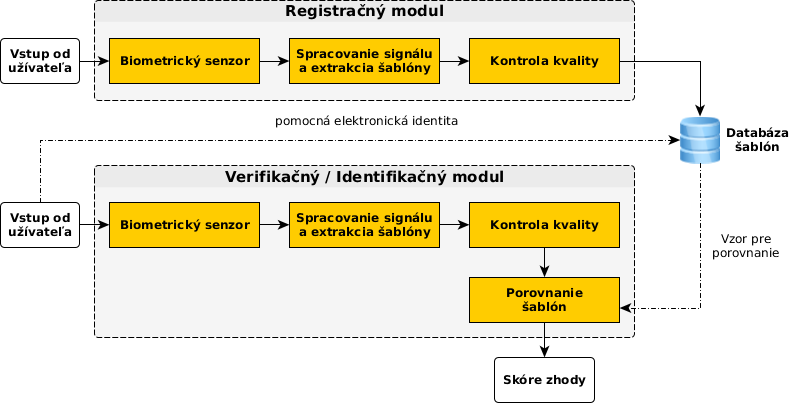
\includegraphics[width=13cm]{img/Bio_system.png}
	\caption{Biometrický systém\cite{bio3}.}
	\label{fig:biosys}
\end{figure}

Výsledkom porovnania verifikačného modulu je miera stotožnenia, alebo zjednodušene \emph{skóre}. Skóre určuje mieru zhody vstupnej vlastnosti verifikačného modulu s jednotlivými šablónami databáze, najvyššie skóre určuje najpodobnejšiu šablónu. V prípade, že také skóre prevyšuje určitú nastavenú hranicu pre chybovosť, \emph{prah}, je možné daný prvok databáze prehlásiť za zhodný a tak určiť alebo potvrdiť identitu uživateľa. 

Biometrický systém môže operovať vo viacerých módoch \cite{bio4}. Tieto módy sú bližie popísané v nasledujúcich podsekciách.

\subsection{Identifikácia}
\emph{Identifikácia} je procesom zisťovania identity osoby, odpovedá na otázku "Kdo to je?" \cite{bio3}. Dochádza pri nej k porovnaniu vstupu s každým prvkom databáze vzorov. Jedná sa teda o porovnanie 1:N \cite{bio}. Cieľom je nájdenie práve jednej zhody za predpokladu, že vstupná identita má svoj vzor v databáze. Prehľadávanie databáze o N prvokoch môže byť časovo náročné, a preto sa často využíva hierarchických systémov zostavených z prvkov databáze, napr. na základe skóre zhody medzi jednotlivými prvkami databáze. Toto usporiadanie následne umožnuje zredukovať hľadanie v databáze len na jej podčasť a skrátiť tak celý proces identifikácie.

Typickým príkladom identifikácie býva identifikácia páchateľa trestného činu na základe jeho odtlačkov prstov nájdených na mieste činu. Získané odtlačky prstov sú porovnané s databázou odtlačkou prstov a pri nájdený zhody je možné identifikovať páchateľa.

\subsection{Verifikácia}
\emph{Verifikácia} je procesom overenia, že užívateľ je naozaj ten, za koho sa vydáva, odpovedá na otázku "Je to naozaj on?" \cite{bio3}. Predstavuje overenie vstupnej vlastnosti voči vybranému vzoru v databáze. Jedná sa teda o porovnanie 1:1 \cite{bio}. Prvok voči ktorému je vstup porovnávaný je buď vopred známy alebo je vyberaný pomocnou identifikáciou z databáze na základe ďalšej (doplnkovej) elektronickej identity, napr. vstupnej karty alebo užívateľského mena a hesla.  Využitie doplnkovej elektronickej identity umožňuje rýchly výber prvku z databáze na rozdiel od identifikácie a poskytuje ďaľšiu úroveň ochrany tým, že útočník potrebuje zfalšovať kombináciu dvoch identifikačných prvkov.

Typickým príkladom verifikácie býva overenie odtlačku prstu užívateľa pri prístupe do mobilného telefónu. Senzor umiestný na telefóne sníma odtačok prstu, ktorý je vzápätí porovnaný s vopred nahraným vzorom a po úspešnej verifikácii je umožnený prístup užívateľa k systému mobilného telefónu.

\section{Hodnotenie výkonnosti biometrických systémov}\label{sec:syscheck}
V predošlej sekcii bol predstavený ideálny model biometrického systému, ktorý nepočíta s chybnou interpretáciou vstupných dát. V praxi sa však často stretávame s tým, že biometrický systém neplní svoju úlohu vždy korektne a na základe využitia systému môže spôsobiť nepríjemnosti v podobe odmietnutia oprávneného užívateľa až po zlyhanie systému v podobe povolenia prístup neoprávnenému útočníkovi.

Z týchto dôvodov boli zavedené nasledujúce charakteristiky, ktoré pomáhajú určiť mieru spoľahlivosti biometrického systému.

\subsection{Miera chybového odmietnutia}
Miera chybového odmietnutia (False-Rejectance Rate = $FRR$) je pravdepodobnosť, že biometrický systém nesprávne vyhodnotí dva vzory náležiace jednej identite ako rozdielne \cite{bio3}. Vyjadruje sa ako podiel počtu nesprávne odmietnutých vstupov k počtu všetkých prijatých vstupov, viď \ref{eq:frr}.
\begin{equation}\label{eq:frr}
FRR = \frac{po\check{c}et \; \mathbf{odmietnut\acute{y}ch} \; porovnan\acute{\imath} \; pri \; zhodn\acute{y}ch \; vzoroch \; u \; subjektu}{celkov\acute{y} \; po\check{c}et \; porovnan\acute{\imath} \; zhodn\acute{y}ch \; vzorov \; subjektu}
\end{equation} 
Prejavom tejto charakteristiky je nesprávne zamietnutý prístup autorizovanému subjektu. U prístupových systémov sú tieto prejavy tolerované do určitej miery, kedže obvykle stačí znovu načítať užívateľský vstup. U policajne-súdnych aplikácií je však táto charakteristika krajne nežiadúca, kedže môže dôjsť k odmietnutiu vzoru a teda identity hľadaného páchateľa.

\subsection{Miera chybového prijatia}
Miera chybového prijatia (False-Acceptance Rate = $FAR$) je pravdepodobnosť, že biometrický systém označí za zhodné dva vzory náležiace k rôznym identitám \cite{bio3}. Vyjadruje sa ako podiel počtu nesprávne prijatých vstupov k počtu všetkých prijatých vstupov, viď \ref{eq:far}.
\begin{equation}\label{eq:far}
FAR = \frac{po\check{c}et \; \mathbf{zhodn\acute{y}ch} \; porovnan\acute{\imath} \; pri \; \mathbf{rozdielnych} \; vzoroch}{celkov\acute{y} \; po\check{c}et \; porovnan\acute{\imath} \; \mathbf{rozdielnych} vzorov}
\end{equation}
Akýkoľvek prejav tejto charakteristiky je veľmi nežiadúci u prístupových systémov, keďže je tak potenciálne umožnení prístup neautorizovanému subjektu.

\subsection{Korekcia variability chýb}
Vyššie uvedené charakteristiky počítaju s faktom, že pomer využitý vo výpočtoch vychádza približne rovnaký pre všetky subjekty. Tento predpoklad však nemusí vždy platiť, a preto je vhodné zamerať sa na ďaľšie detaily, ktoré vplývajú na chybovosť biometrického systému \cite{bio3}.

\emph{Miera zlyhania pridania užívateľa (Failure To Enroll Rate = $FTE$)} -- pravdepodobnosť zlyhania procesu vkladania novej užívateľskej identity do biometrického systému.
\emph{Miera zlyhania získania vstupu (Failure To Aquire Rate = $FTA$)} -- pravdepodobnosť, že získaný vstup nebude vhodný pre využitie pre identifikáciu, či verifikáciu, napr. z dôvodu nedostatočnej kvality vstupu.
\emph{Miera chybnej zhody (False Match Rate = $FMR$)} -- zhruba sa zhoduje s $FAR$, avšak rozdiel je vo využití pokusov pre výpočet $FMR$, bez ohľadu na to, od ktorého užívateľa dané pokusy vzišli. Zatiaľ čo $FAR$ využíva transakcí, ktoré sa môžu skladať z viacerých pokusov, pričom sa berie ohľad i na úspešnosť prijatia vstupu ovplyvnenú $FTE$ a $FTA$.
\emph{Miera chybnej nezhody (False Non-Match Rate = $FNMR$)} -- zhruba sa zhoduje s $FRR$, s obdobným rozdielom ako je uvedené u $FMR$.

S pomocou týchto charakteristík môžeme vyjadriť $FAR(n)$ a $FRR(n)$ v rovniciach, kde jedna transakcia $n$ pozostáva z jediného pokusu, viď \ref{eq:frrn} a \ref{eq:farn}.
\begin{align}
FRR(n) = FTE + FTA + FNMR(n) \label{eq:frrn} \\
FAR(n) = (1-FTE) * (1-FTA) * FMR(n) \label{eq:farn}
\end{align}

Spriemerovaní naprieč všetkými $N$ transakciami dostaneme výsledné $FAR$ a $FRR$, viď \ref{eq:gfrr} a \ref{eq:gfar}.
\begin{align}
FRR = \frac{1}{N}\sum{n=1}{N} FRR(n) \label{eq:gfrr} \\
FAR = \frac{1}{N}\sum{n=1}{N} FMR(n) \label{eq:gfar}
\end{align}

\subsection{Vyhodnotenie a nastavenie biometrického systému}
Z charakteristík uvedených vyššie vyplýva, že ideálny biometrický systém by mal dosahovať $FAR$ a $FRR$ rovné 0. Je preto nutné systém optimalizovať, aby poskytoval čo možno najpresnejšie výsledky. 

Táto optimalizácia je realizovateľná vďaka možnosti nastavenia \emph{prahu citlivosti} pre skóre vstupu u biometrického systému \cite{bio3}. Je tak možné ovplyvniť prijatie, či odmietnutie vstupu, čo má priamy dopad na $FAR$ a $FRR$. Pre prípad, že je miera $FAR$ i $FRR$ chýb vyrovnaná, teda $FAR = FRR$, sa zaužíval pojem $EER$ -- \emph{Equal Error Rate}.

\begin{figure}[!ht]
	\centering
	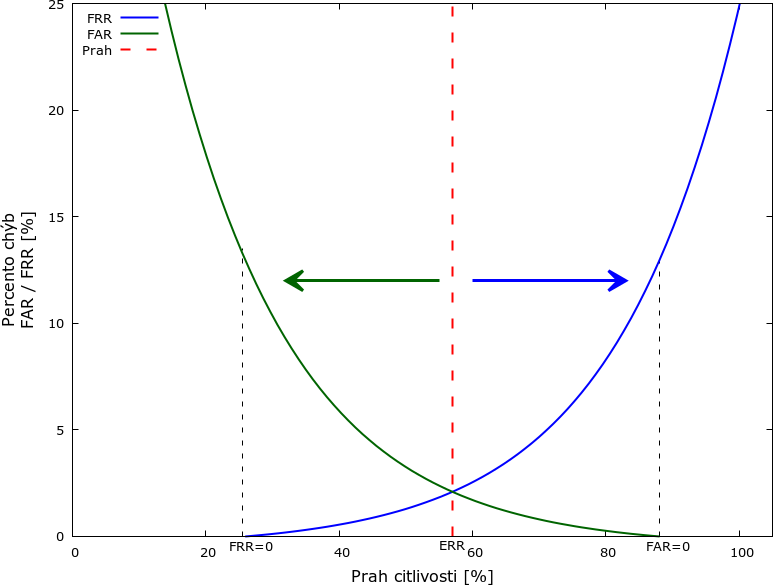
\includegraphics[width=13cm]{img/prah.png}
	\caption{Nastavenie prahu citlivosti\cite{bio3}.}
	\label{fig:prah}
\end{figure}

Obrázok \ref{fig:prah} približuje problematiku nastavovania prahu biometrického systému. Nastavením prahu pre zníženie $FAR$ (v smere modrej šípky) dosiahneme zvýšenej bezpečnosti, avšak zároveň zvyšujeme pravdepodobnosť odmietnutia oprávneného užívateľa $FRR$. V prípade nastavenia prahu pre zníženie $FRR$, je kompromitovaná bezpečnosť v podobe zvýšeného $FAR$.

V praxi je teda bohužial nemožné dosiahnuť nulové $FAR$ i $FRR$ zároveň, keďže bezchybný systém neexistuje. Je teda zrejmé, že nastavenie prahu priamo súvisí s využitím biometrického systému. Pri hľadaní páchateľa v databáze je neprijateľné jeho prehliadnutie a $FRR$ je preto potrebné nastaviť na 0. Nesprávne identifikované osoby možu byť neskôr ručne vylúčené. Naopak u prístupových systémov je neprijateľné, aby bol umožnený prístup neoprávnenej osobe a tak naopak $FAR$ musí dosahovať nulovej hodnoty. Neprijatie oprávneného užívateľa je u prístupového systému len otázkou komfortu a užívateľ môže opakovať zadanie vstupu \cite{bio3}.

Navyše priebehy $FAR$ a $FRR$ nie sú v praxi tak plynulé ako je naznačené na obrázku \ref{fig:prah}. Vyhodnotenie výkonnosti daného biometrického systému teda nie je možné len na základe minimálnych či maximálnych hodnôt $FRR$ a $FAR$, ale je potrebná znalosť priebehu oboch veličín. Ich kombináciou dosiahneme vhodnú charakteristiku a zjednodušíme porovnávanie.

Vyjadrenie vzťahu $FRR$ a $FAR$ sa prevádza pomocou $DET$ krivky (Detection Error Trade-off), viď obrázok \ref{fig:det}. Charakteristiky $FRR$ a $FAR$ uvedené v predošlých kapitolách sú zanesené do grafu a porovnané voči sebe.

\begin{figure}[h]
	\centering
	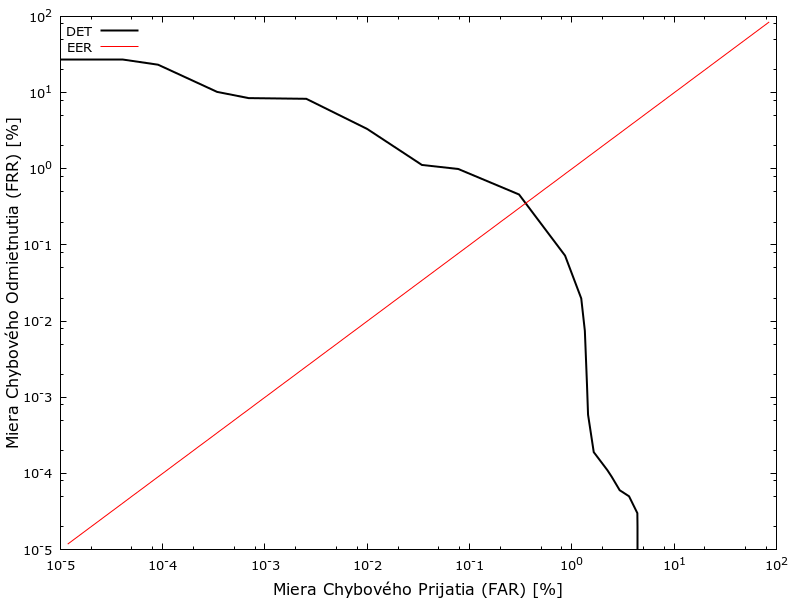
\includegraphics[width=13cm]{img/det.png}
	\caption{$DET$ krivka\cite{bio}.}
	\label{fig:det}
\end{figure}

Častejšie sa však stretneme s podobnou krivkou porovnávajúcou charakteristiky $FAR$ a $1 - FRR$, zvanou $ROC$ (Receiver Operating Characteristic alebo Curve), viď obrázok \ref{fig:roc}. Miera $1 - FRR$ vyjadruje mieru prijatia korektných (autorizovaných) vstupov a môžeme ju tiež nazvať $TAR$ (True Acceptance Rate).

\begin{figure}[h]
	\centering
	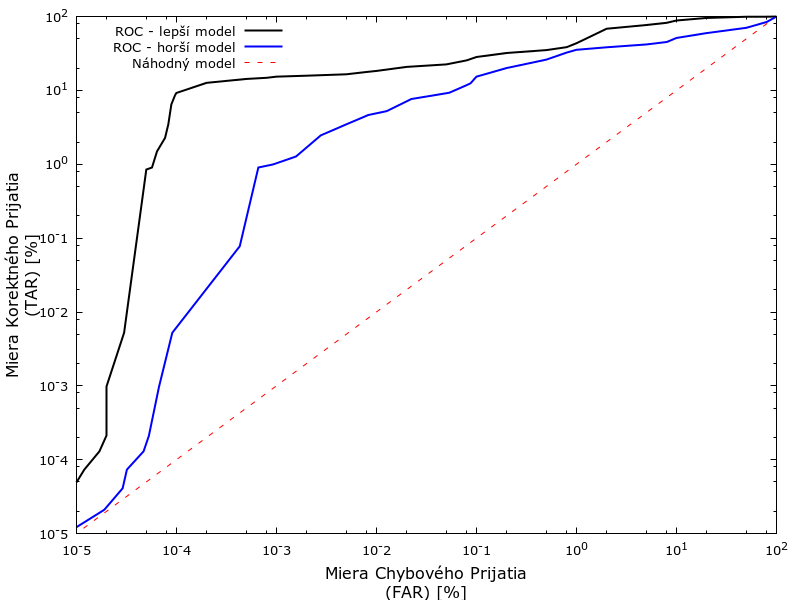
\includegraphics[width=13cm]{img/roc.png}
	\caption{$ROC$ krivka\cite{bio}.}
	\label{fig:roc}
\end{figure}

Keďže obe krivky sú typicky veľmi blízko osí súradného systému, pre názorné porovnanie viacerých systémov sa používa logaritmické zobrazenie, ako je znázornené na obrázkoch. 

V prípade $ROC$ leží ideálny systém v bode $TAR = 1$ a $FAR = 0$, cieľom je priblížiť sa k tomuto bodu, ale tak, aby účel systému nebol kompromitovaný. To znamená, že ak je účelom identifikácia, snaha bude pravdepodobne udržať krivku čo najbližšie osi x, t.j. $FAR$, zatiaľ čo u verifikácie je pravdepodobne snaha udržať krivku čo najbližšie osi y, t.j. $TAR$.

Závislosť $FAR$ a $TAR$ vyjadrená $ROC$ krivkou vyjadruje schopnosti biometrického systému bez skreslenia voľbou konkrétneho prahu. Krivka $ROC$ je teda objektívnym prostriedkom pre porovnanie výkonnosti rôznych biometrických systémov.

\chapter{Orgán zraku}\label{ch:kap1}
Orgán zraku je primárny párový senzorický orgán ľudského tela, vďaka ktorému sa človek dokáže jednoducho orientovať v okolitom priestore. Zrakom vnímame až 90\% informácií z okolitého prostredia, a preto je tento orgán Strategické umiestnenie tohoto orgánu na hlave (blízko mozgu) ho robí ľahko dostupným pre použitie v biometrii.

Táto kapitola rozoberá základné poznatky týkajúce sa orgánu zraku, rozoberá jeho optické vlastnosti a zavádza pojmy, ktoré sú využívané v nasledujúcich kapitolách.

\section{Zloženie oka}\label{sec:oko}
Oko, očná bulva, má takmer sférický tvar. Vďaka tomuto tvaru je jeho pohyb v očnej jamke rýchly a zabezpečuje zameranie sa na objekt záujmu v zlomku sekundy \cite{bio4}.
Zloženie oka umožňuje jednoduchý priestup svetla s minimálnymi , obmedzenie množstva svetla v prípade zvýšeného jasu a jeho zaostrenie na sietnicu.

\begin{figure}[h]
  \centering
  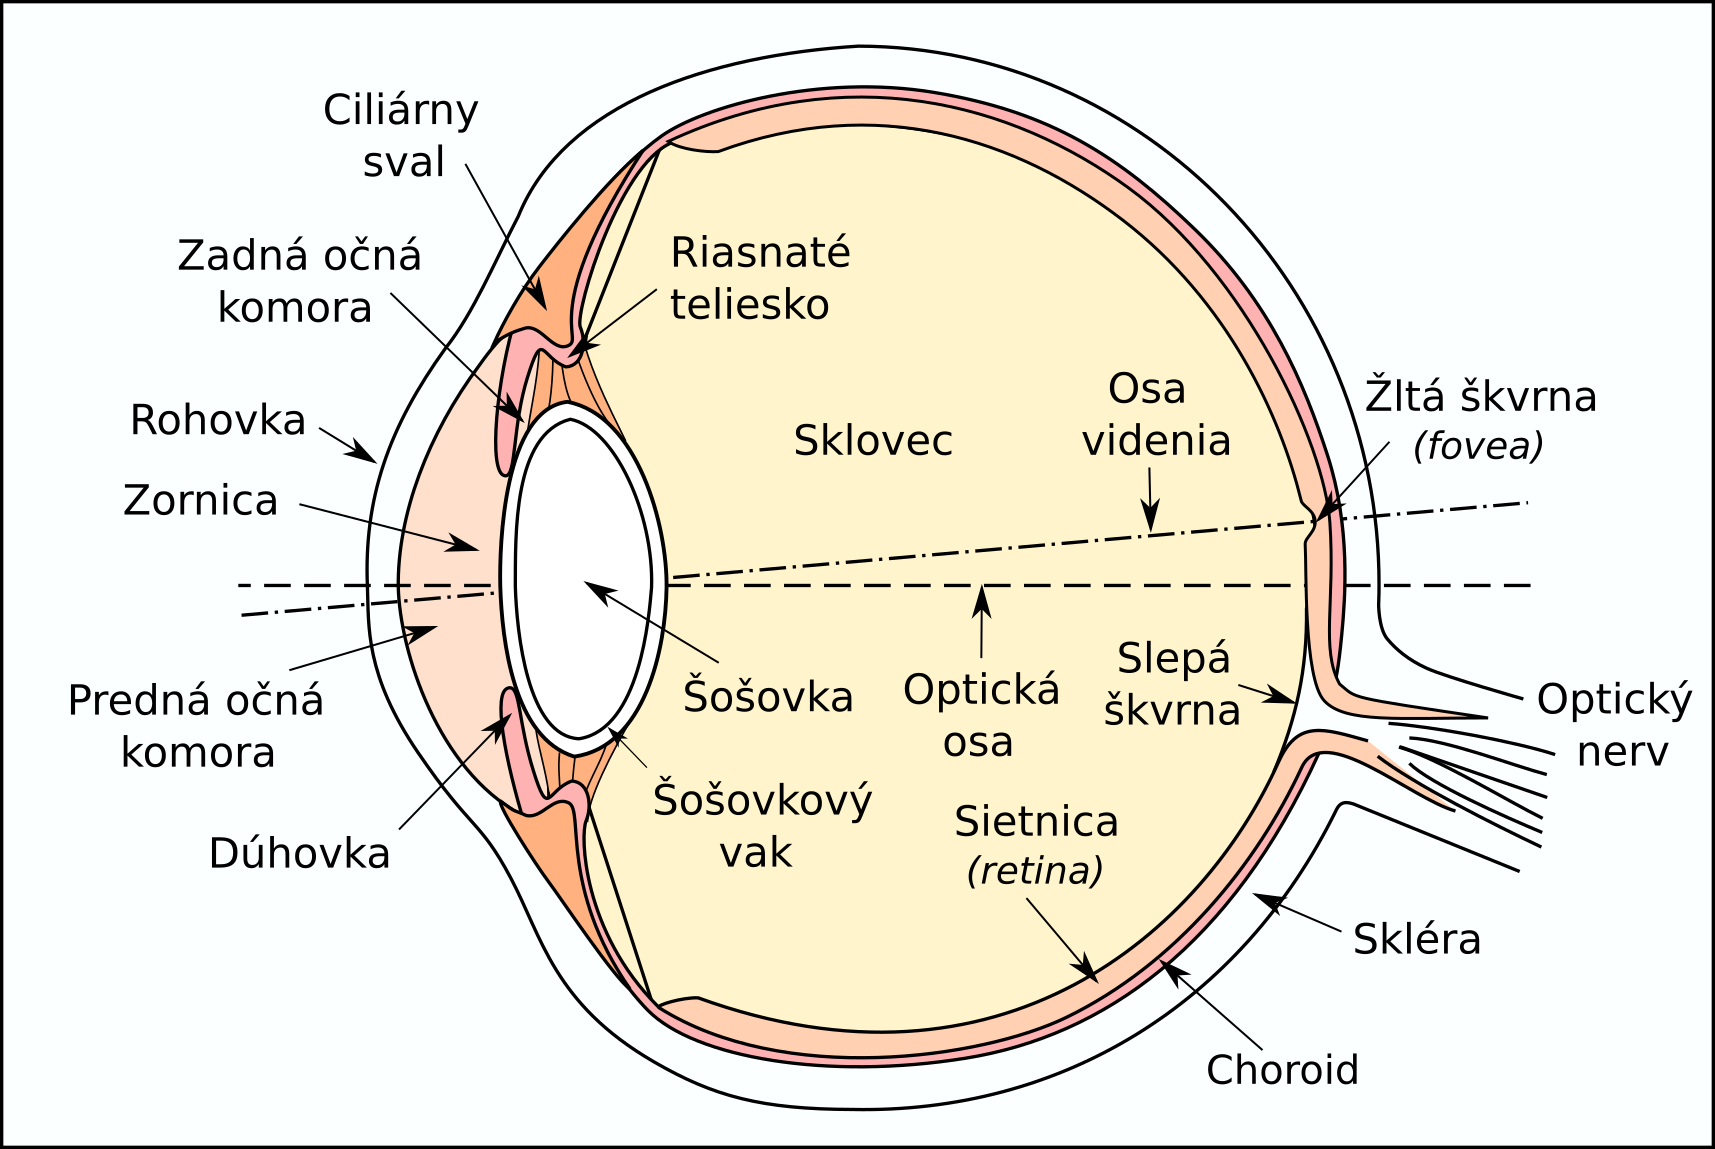
\includegraphics[width=11cm]{img/Eyesection.png}
  \caption{Štruktúra ľudského oka\cite{retina}}
  \label{fig:retina}
\end{figure}

Svetlo pri priechode okom prechádza nasledujúcimi prvkami\cite{zloz_oka}:
\begin{itemize}
\item \textbf{rohovka} (cornea) -- transparentná vrstva v prednej časti oka chrániaca miesto vstupu svetla do oka. Je vysoko odolná a má značné regeneračné vlastnosti.
\item \textbf{predná a zadná očná komora} -- obsahujú číru tekutinu, ktorá vypĺňa priestor za rohovkou až k dúhovke a šošovke (v mieste zornice). Udržujú stály očný tlak, zásobujú rohovku, šošovku a okolité tkanivá živinami\cite{zmysly}.
\item \textbf{šošovka} -- elastický útvar bikonvexného tvaru. Je zavesená na tenkých vláknach a napínaná ciliárnym svalom, ktorý tak upravuje optickú mohutnosť šošovky a umožňuje zaostrovanie, akomodáciu.
\item \textbf{sklovec} -- číry gél vypĺňajúci dutinu oka za šošovkou.
\item \textbf{sietnica} (retina) -- viacvrstvá štruktúra obsahujúca svetlocitlivé bunky. Elektrický impulz generovaný svetlocitlivými bunkami je prenášaný sieťou komplexných nervových dráh až do mozgu.
\end{itemize}

Každý z týchto prvkov má vlastnosti, ktoré sa podieľajú na správnom prenose svetla k sietnici. 


- popis ako je svetlo ovplyvnene prvkami oka
- popis ako sa obraz dostava na sietnicu

- popis kde je sietnica a na co sluzi \cite{vlast_oka}
- potrebujes sa dostat k popisu klucovych prvkov sietnice

- 

- jednotlive casti oka a ich nazov podla odbornej literatury
- popis priepustnosti svetla skrz oko a vlastnosti svetla ktore zachytava sietnica
- odkaz na choroby ktore niesu spojene priamo so sietnicou?

\section{Sietnica}\label{sec:sietnica}
- skladba sietnice, rieciste, svetlocitlive bunky, popis jednotlivych prvkov na sietnici
- reakcia svetlocitlivych buniek na svetlo, ich rozlozenie po sietnici
- 

\section{Biometria sietnice}\label{sec:bioret}

\chapter{Patológia sietnice}\label{ch:kap2}
TBD\cite{prim}
\section{TBD}
TBD\cite{sec}
TBD\cite{bio}

\chapter{Zdroje vstupných dát}\label{ch:kap3}
- popis jednotlive databaze a ich parametry - vyuzi existujuce prace a zosumarizuj data!!!

\chapter{Detekcia a korekcia nálezov}\label{ch:kap4}

\chapter{Implementácia algoritmu}

\chapter{Systém testovania a výsledky}\label{ch:kap5}

\chapter{Záver}\label{ch:kap6}
Závěrečná kapitola obsahuje zhodnocení dosažených výsledků se zvlášť vyznačeným vlastním přínosem studenta. Povinně se zde objeví i zhodnocení z pohledu dalšího vývoje projektu, student uvede náměty vycházející ze zkušeností s řešeným projektem a uvede rovněž návaznosti na právě dokončené projekty.

%=========================================================================
 % viz. obsah.tex / see obsah.tex

  % Pouzita literatura / Bibliography
  % ----------------------------------------------
\ifslovak
  \makeatletter
  \def\@openbib@code{\addcontentsline{toc}{chapter}{Literatúra}}
  \makeatother
  \bibliographystyle{bib-styles/slovakiso}
\else
  \ifczech
    \makeatletter
    \def\@openbib@code{\addcontentsline{toc}{chapter}{Literatura}}
    \makeatother
    \bibliographystyle{bib-styles/czechiso}
  \else 
    \makeatletter
    \def\@openbib@code{\addcontentsline{toc}{chapter}{Bibliography}}
    \makeatother
    \bibliographystyle{bib-styles/englishiso}
  %  \bibliographystyle{alpha}
  \fi
\fi
  \begin{flushleft}
  \bibliography{DIP_xvavro00-20-literatura-bibliography}
  \end{flushleft}

  % vynechani stranky v oboustrannem rezimu
  % Skip the page in the two-sided mode
  \iftwoside
    \cleardoublepage
  \fi

  % Prilohy / Appendices
  % ---------------------------------------------
  \appendix
\ifczech
  \renewcommand{\appendixpagename}{Přílohy}
  \renewcommand{\appendixtocname}{Přílohy}
  \renewcommand{\appendixname}{Příloha}
\fi
\ifslovak
  \renewcommand{\appendixpagename}{Prílohy}
  \renewcommand{\appendixtocname}{Prílohy}
  \renewcommand{\appendixname}{Príloha}
\fi
  \appendixpage

% vynechani stranky v oboustrannem rezimu
% Skip the page in the two-sided mode
\iftwoside
  \cleardoublepage
\fi
  
\ifslovak
%  \section*{Zoznam príloh}
%  \addcontentsline{toc}{section}{Zoznam príloh}
\else
  \ifczech
%    \section*{Seznam příloh}
%    \addcontentsline{toc}{section}{Seznam příloh}
  \else
%    \section*{List of Appendices}
%    \addcontentsline{toc}{section}{List of Appendices}
  \fi
\fi
  \startcontents[chapters]
  % seznam příloh / list of appendices
  % \printcontents[chapters]{l}{0}{\setcounter{tocdepth}{2}}
  
  % vynechani stranky v oboustrannem rezimu
  \iftwoside
    \cleardoublepage
  \fi
  % Tento soubor nahraďte vlastním souborem s přílohami (nadpisy níže jsou pouze pro příklad)
% This file should be replaced with your file with an appendices (headings below are examples only)

% Umístění obsahu paměťového média do příloh je vhodné konzultovat s vedoucím
% Placing of table of contents of the memory media here should be consulted with a supervisor
%\chapter{Obsah přiloženého paměťového média}

%\chapter{Manuál}

%\chapter{Konfigurační soubor} % Configuration file

%\chapter{RelaxNG Schéma konfiguračního souboru} % Scheme of RelaxNG configuration file

%\chapter{Plakát} % poster

\chapter{Jak pracovat s touto šablonou}
\label{jak}

V této kapitole je uveden popis jednotlivých částí šablony, po kterém následuje stručný návod, jak s touto šablonou pracovat. 

Jedná se o přechodnou verzi šablony. Nová verze bude zveřejněna do konce roku 2016 a bude navíc obsahovat nové pokyny ke správnému využití šablony, závazné pokyny k~vypracování bakalářských a diplomových prací (rekapitulace pokynů, které jsou dostupné na~webu) a nezávazná doporučení od vybraných vedoucích. Jediné soubory, které se v nové verzi změní, budou projekt-01-kapitoly-chapters.tex a projekt-30-prilohy-appendices.tex, jejichž obsah každý student vymaže a nahradí vlastním. Šablonu lze tedy bez problémů využít i~v~současné verzi.

\section*{Popis částí šablony}

Po rozbalení šablony naleznete následující soubory a adresáře:
\begin{DESCRIPTION}
  \item [bib-styles] Styly literatury (viz níže). 
  \item [obrazky-figures] Adresář pro Vaše obrázky. Nyní obsahuje placeholder.pdf (tzv. TODO obrázek, který lze použít jako pomůcku při tvorbě technické zprávy), který se s prací neodevzdává. Název adresáře je vhodné zkrátit, aby byl jen ve zvoleném jazyce.
  \item [template-fig] Obrázky šablony (znak VUT).
  \item [fitthesis.cls] Šablona (definice vzhledu).
  \item [Makefile] Makefile pro překlad, počítání normostran, sbalení apod. (viz níže).
  \item [projekt-01-kapitoly-chapters.tex] Soubor pro Váš text (obsah nahraďte).
  \item [projekt-20-literatura-bibliography.bib] Seznam literatury (viz níže).
  \item [projekt-30-prilohy-appendices.tex] Soubor pro přílohy (obsah nahraďte).
  \item [projekt.tex] Hlavní soubor práce -- definice formálních částí.
\end{DESCRIPTION}

Výchozí styl literatury (czechiso) je od Ing. Martínka, přičemž anglická verze (englishiso) je jeho překladem s drobnými modifikacemi. Oproti normě jsou v něm určité odlišnosti, ale na FIT je dlouhodobě akceptován. Alternativně můžete využít styl od Ing. Radima Loskota nebo od Ing. Radka Pyšného\footnote{BP Ing. Radka Pyšného \url{http://www.fit.vutbr.cz/study/DP/BP.php?id=7848}}. Alternativní styly obsahují určitá vylepšení, ale zatím nebyly řádně otestovány větším množstvím uživatelů. Lze je považovat za beta verze pro zájemce, kteří svoji práci chtějí mít dokonalou do detailů a neváhají si nastudovat detaily správného formátování citací, aby si mohli ověřit, že je vysázený výsledek v pořádku.

Makefile kromě překladu do PDF nabízí i další funkce:
\begin{itemize}
  \item přejmenování souborů (viz níže),
  \item počítání normostran,
  \item spuštění vlny pro doplnění nezlomitelných mezer,
  \item sbalení výsledku pro odeslání vedoucímu ke kontrole (zkontrolujte, zda sbalí všechny Vámi přidané soubory, a případně doplňte).
\end{itemize}

Nezapomeňte, že vlna neřeší všechny nezlomitelné mezery. Vždy je třeba manuální kontrola, zda na konci řádku nezůstalo něco nevhodného -- viz Internetová jazyková příručka\footnote{Internetová jazyková příručka \url{http://prirucka.ujc.cas.cz/?id=880}}.

\paragraph {Pozor na číslování stránek!} Pokud má obsah 2 strany a na 2. jsou jen \uv{Přílohy} a~\uv{Seznam příloh} (ale žádná příloha tam není), z nějakého důvodu se posune číslování stránek o 1 (obsah \uv{nesedí}). Stejný efekt má, když je na 2. či 3. stránce obsahu jen \uv{Literatura} a~je možné, že tohoto problému lze dosáhnout i jinak. Řešení je několik (od~úpravy obsahu, přes nastavení počítadla až po sofistikovanější metody). \textbf{Před odevzdáním proto vždy překontrolujte číslování stran!}


\section*{Doporučený postup práce se šablonou}

\begin{enumerate}
  \item \textbf{Zkontrolujte, zda máte aktuální verzi šablony.} Máte-li šablonu z předchozího roku, na stránkách fakulty již může být novější verze šablony s~aktualizovanými informacemi, opravenými chybami apod.
  \item \textbf{Zvolte si jazyk}, ve kterém budete psát svoji technickou zprávu (česky, slovensky nebo anglicky) a svoji volbu konzultujte s vedoucím práce (nebyla-li dohodnuta předem). Pokud Vámi zvoleným jazykem technické zprávy není čeština, nastavte příslušný parametr šablony v souboru projekt.tex (např.: \verb|documentclass[english]{fitthesis}| a přeložte prohlášení a poděkování do~angličtiny či slovenštiny.
  \item \textbf{Přejmenujte soubory.} Po rozbalení je v šabloně soubor projekt.tex. Pokud jej přeložíte, vznikne PDF s technickou zprávou pojmenované projekt.pdf. Když vedoucímu více studentů pošle projekt.pdf ke kontrole, musí je pracně přejmenovávat. Proto je vždy vhodné tento soubor přejmenovat tak, aby obsahoval Váš login a (případně zkrácené) téma práce. Vyhněte se však použití mezer, diakritiky a speciálních znaků. Vhodný název tedy může být např.: \uv{xlogin00-Cisteni-a-extrakce-textu.tex}. K přejmenování můžete využít i přiložený Makefile:
\begin{verbatim}
make rename NAME=xlogin00-Cisteni-a-extrakce-textu
\end{verbatim}
  \item Vyplňte požadované položky v souboru, který byl původně pojmenován projekt.tex, tedy typ, rok (odevzdání), název práce, svoje jméno, ústav (dle zadání), tituly a~jméno vedoucího, abstrakt, klíčová slova a další formální náležitosti.
  \item Nahraďte obsah souborů s kapitolami práce, literaturou a přílohami obsahem svojí technické zprávy. Jednotlivé přílohy či kapitoly práce může být výhodné uložit do~samostatných souborů -- rozhodnete-li se pro toto řešení, je doporučeno zachovat konvenci pro názvy souborů, přičemž za číslem bude následovat název kapitoly. 
  \item Nepotřebujete-li přílohy, zakomentujte příslušnou část v projekt.tex a příslušný soubor vyprázdněte či smažte. Nesnažte se prosím vymyslet nějakou neúčelnou přílohu jen proto, aby daný soubor bylo čím naplnit. Vhodnou přílohou může být obsah přiloženého paměťového média.
  \item Nascanované zadání uložte do souboru zadani.pdf a povolte jeho vložení do práce parametrem šablony v projekt.tex (\verb|documentclass[zadani]{fitthesis}|).
  \item Nechcete-li odkazy tisknout barevně (tedy červený obsah -- bez konzultace s vedoucím nedoporučuji), budete pro tisk vytvářet druhé PDF s tím, že nastavíte parametr šablony pro tisk: (\verb|documentclass[zadani,print]{fitthesis}|).  Barevné logo se nesmí tisknout černobíle!
  \item Vzor desek, do kterých bude práce vyvázána, si vygenerujte v informačním systému fakulty u zadání. Pro disertační práci lze zapnout parametrem v šabloně (více naleznete v souboru fitthesis.cls).
  \item Nezapomeňte, že zdrojové soubory i (obě verze) PDF musíte odevzdat na CD či jiném médiu přiloženém k technické zprávě.
\end{enumerate}

\subsection*{Pokyny pro oboustranný tisk}
\begin{itemize}
\item Zapíná se parametrem šablony: \verb|\documentclass[twoside]{fitthesis}|
\item Po vytištění oboustranného listu zkontrolujte, zda je při prosvícení sazební obrazec na obou stranách na stejné pozici. Méně kvalitní tiskárny s duplexní jednotkou mají často posun o 1--3 mm. Toto může být u některých tiskáren řešitelné tak, že vytisknete nejprve liché stránky, pak je dáte do stejného zásobníku a vytisknete sudé.
\item Za titulním listem, obsahem, literaturou, úvodním listem příloh, seznamem příloh a případnými dalšími seznamy je třeba nechat volnou stránku, aby následující část začínala na liché stránce (\textbackslash cleardoublepage).
\item  Konečný výsledek je nutné pečlivě překontrolovat.
\end{itemize}


\subsection*{Užitečné nástroje}
\label{nastroje}

Následující seznam není výčtem všech využitelných nástrojů. Máte-li vyzkoušený osvědčený nástroj, neváhejte jej využít. Pokud však nevíte, který nástroj si zvolit, můžete zvážit některý z následujících:

\begin{description}
	\item[\href{http://miktex.org/download}{MikTeX}] \LaTeX{} pro Windows -- distribuce s jednoduchou instalací a vynikající automatizací stahování balíčků.
	\item[\href{http://texstudio.sourceforge.net/}{TeXstudio}] Přenositelné opensource GUI pro \LaTeX{}.  Ctrl+klik umožňuje přepínat mezi zdrojovým textem a PDF. Má integrovanou kontrolu pravopisu, zvýraznění syntaxe apod. Pro jeho využití je nejprve potřeba nainstalovat MikTeX.
	\item[\href{http://jabref.sourceforge.net/download.php}{JabRef}] Pěkný a jednoduchý program v Javě pro správu souborů s bibliografií (literaturou). Není potřeba se nic učit -- poskytuje jednoduché okno a formulář pro editaci položek.
	\item[\href{https://inkscape.org/en/download/}{InkScape}] Přenositelný opensource editor vektorové grafiky (SVG i PDF). Vynikající nástroj pro tvorbu obrázků do odborného textu. Jeho ovládnutí je obtížnější, ale výsledky stojí za to.
	\item[\href{https://git-scm.com/}{GIT}] Vynikající pro týmovou spolupráci na projektech, ale může výrazně pomoci i jednomu autorovi. Umožňuje jednoduché verzování, zálohování a přenášení mezi více počítači.
	\item[\href{http://www.overleaf.com/}{Overleaf}] Online nástroj pro \LaTeX{}. Přímo zobrazuje náhled a umožňuje jednoduchou spolupráci (vedoucí může průběžně sledovat psaní práce), vyhledávání ve zdrojovém textu kliknutím do PDF, kontrolu pravopisu apod. Zdarma jej však lze využít pouze s určitými omezeními (někomu stačí na disertaci, jiný na ně může narazit i při psaní bakalářské práce) a pro dlouhé texty je pomalejší.
\end{description}

\subsection*{Užitečné balíčky pro \LaTeX}

Studenti při sazbě textu často řeší stejné problémy. Některé z nich lze vyřešit následujícími balíčky pro \LaTeX:

\begin{itemize}
  \item \verb|amsmath| -- rozšířené možnosti sazby rovnic,
  \item \verb|float, afterpage, placeins| -- úprava umístění obrázků,
  \item \verb|fancyvrb, alltt| -- úpravy vlastností prostředí Verbatim, 
  \item \verb|makecell| -- rozšíření možností tabulek,
  \item \verb|pdflscape, rotating| -- natočení stránky o 90 stupňů (pro obrázek či tabulku),
  \item \verb|hyphenat| -- úpravy dělení slov,
  \item \verb|picture, epic, eepic| -- přímé kreslení obrázků.
\end{itemize}

Některé balíčky jsou využity přímo v šabloně (v dolní části souboru fitthesis.cls). Nahlédnutí do jejich dokumentace může být rovněž užitečné.

Sloupec tabulky zarovnaný vlevo s pevnou šířkou je v šabloně definovaný \uv{L} (používá se jako \uv{p}).

 % viz. prilohy.tex / see prilohy.tex
\end{document}
